\subsection{Manager}\label{sec:runtime_manager}

Manager dienen in \textit{helios} der Orchestrierung verschiedener Aktionen innerhalb der \textit{GameLoop}; ihr Konzept ist dabei nicht an eine bestimmte Fachlichkeit gebunden.
Sie werden häufig als \texttt{CommandHandler} eingesetzt, womit ihnen die Aufgabe zukommt, innerhalb eines Frames Befehle zu sammeln und diese zu einem bestimmten Zeitpunkt - der von der \textit{GameLoop} ausgelöst und an \texttt{GameWorld::flushManagers()} signalisiert wird - zusammen mit den damit verbundenen Aufgaben auszuführen.\\

Zur Identifizierung eines Types, der die Rolle eines \textit{Managers} in \textit{helios} besitzen kann, werden \texttt{Concepts} (\texttt{IsManagerLike}) zusammen mit der \texttt{EngineRoleTag} ``\texttt{ManagerRole}`` zur Kennzeichnung verwendet.

\textit{helios} implementiert u.\,a. folgende Manager:

\begin{itemize}
    \item \texttt{HealthManager}: Verarbeitet Befehle zur Anwendung von Schaden auf die in der \textit{GameWorld} aktiven \texttt{GameObject}s, bspw. ausgelöst durch Kollisionen.
    Aktualisierungen der \texttt{HealthComponent} der betreffenden Objekte werden dabei über Events an die nächste Phase kommuniziert, was eine Verarbeitung als grafische Effekte oder Audio-Elemente erlaubt.
    Der Manager sorgt außerdem dafür, dass die Objekte eine \texttt{DeadTagComponent} erhalten, um bestimmte Systeme (wie Bewegungssysteme) nicht mehr innerhalb desselben Frames zu berücksichtigen.
    \item \texttt{ScorePoolManager}: Verwaltet die \texttt{ScorePools} in \textit{helios}, die dafür verwendet werden, Punkte bzw. Belohnungen zu sammeln.
    Die \texttt{ScorePools} sind abstrakte Punktesysteme, die klassische Punktestände repräsentieren können und über \texttt{ScorePoolId}s an \texttt{GameObject}s gebunden werden können, sodass verschiedene \texttt{GameObject}s über eigene, voneinander getrennte Punktestände verfügen.
    Dies erlaubt beispielsweise auch die Berechnung von Erfahrungspunkten über einen solchen Pool.
    Das eigentliche Scoring ist als Mechanik in \texttt{helios.engine.mechanics.scoring} implementiert; der Manager integriert diese auf breiter Ebene in die \textit{GameWorld}.

    \item \texttt{GameObjectPoolManager}: Verwaltet verschiedene Objektpools von \texttt{GameObject}s, um die Erstellung solcher Entitäten zur Laufzeit möglichst zu vermeiden.
    Der Manager bedient sich hierbei einer Liste von \texttt{PoolConfiguration}s, die jeweils eine festgelegte Zahl von \texttt{GameObject}s auf Basis eines Prefabs  enthalten, und bietet Fassadenfunktionen zur Rückgabe und Bereitstellung der in den Pools enthaltenen Objekte an (\texttt{acquire()}, \texttt{release()}).
     Entgegen vieler anderer Manager, die auch als \texttt{CommandHandler} fungieren, arbeitet der \texttt{GameObjectPoolManager} nicht selbst als Befehlsverarbeiter zur Verwaltung der Objekte in den Pools - diese Rolle wird von dem im Folgenden vorgestellten Manager übernommen, dem \texttt{SpawnManager}.

    \item \texttt{SpawnManager}: Auf Basis verschiedener Regeln und Bedingungen hat dieser Manager die Aufgabe, \texttt{GameObject}s in die Spielwelt zu spawnen (\texttt{SpawnCommand}), oder diese wegzuräumen und sie in die \texttt{GamePool}s zurückzulegen (\texttt{DespawnCommand}).
    Hierzu besitzt der \texttt{SpawnManager} eine Assoziation zu dem in der Runtime genutzten \texttt{GameObjectPoolManager}, damit an diesen die Ressourcenverwaltung übertragen werden kann.
    Ist eine Entität nicht mi einem Pool verbunden, findet an dieser Stelle folglich keine Delegation statt

    \item \texttt{StateManager}: Eine besondere Verantwortung besitzt der \texttt{StateManager}, der die Verwaltung der verschiedenen Spielzustände (\textit{States}) übernimmt.
    Auf das \textit{State Management} gehen wir kurz als gesondertes Konzept in Abschnitt~\ref{sec:state_management} ein.
\end{itemize}

Daneben finden sich noch der \texttt{WorldLifecycleManager} zur Verwaltung von Lifecycle-Commands wie einem \texttt{reset()} der \textit{GameWorld}, der \texttt{TimerManager} zur Verwaltung von Spielmechaniken, die eine Zeitmessung benötigen, sowie der \texttt{UiActionCommandManager} zur Verarbeitung von UI-Commands (wie der Aktivierung von Menüoptionen).\\

Abbildung~\ref{fig:manager_auswirkungen} zeigt den Ausschnitt einer Spielszene, wobei die von den Managern beeinflussten Systeme markiert sind.

\begin{figure}[htbp]
    \centering
    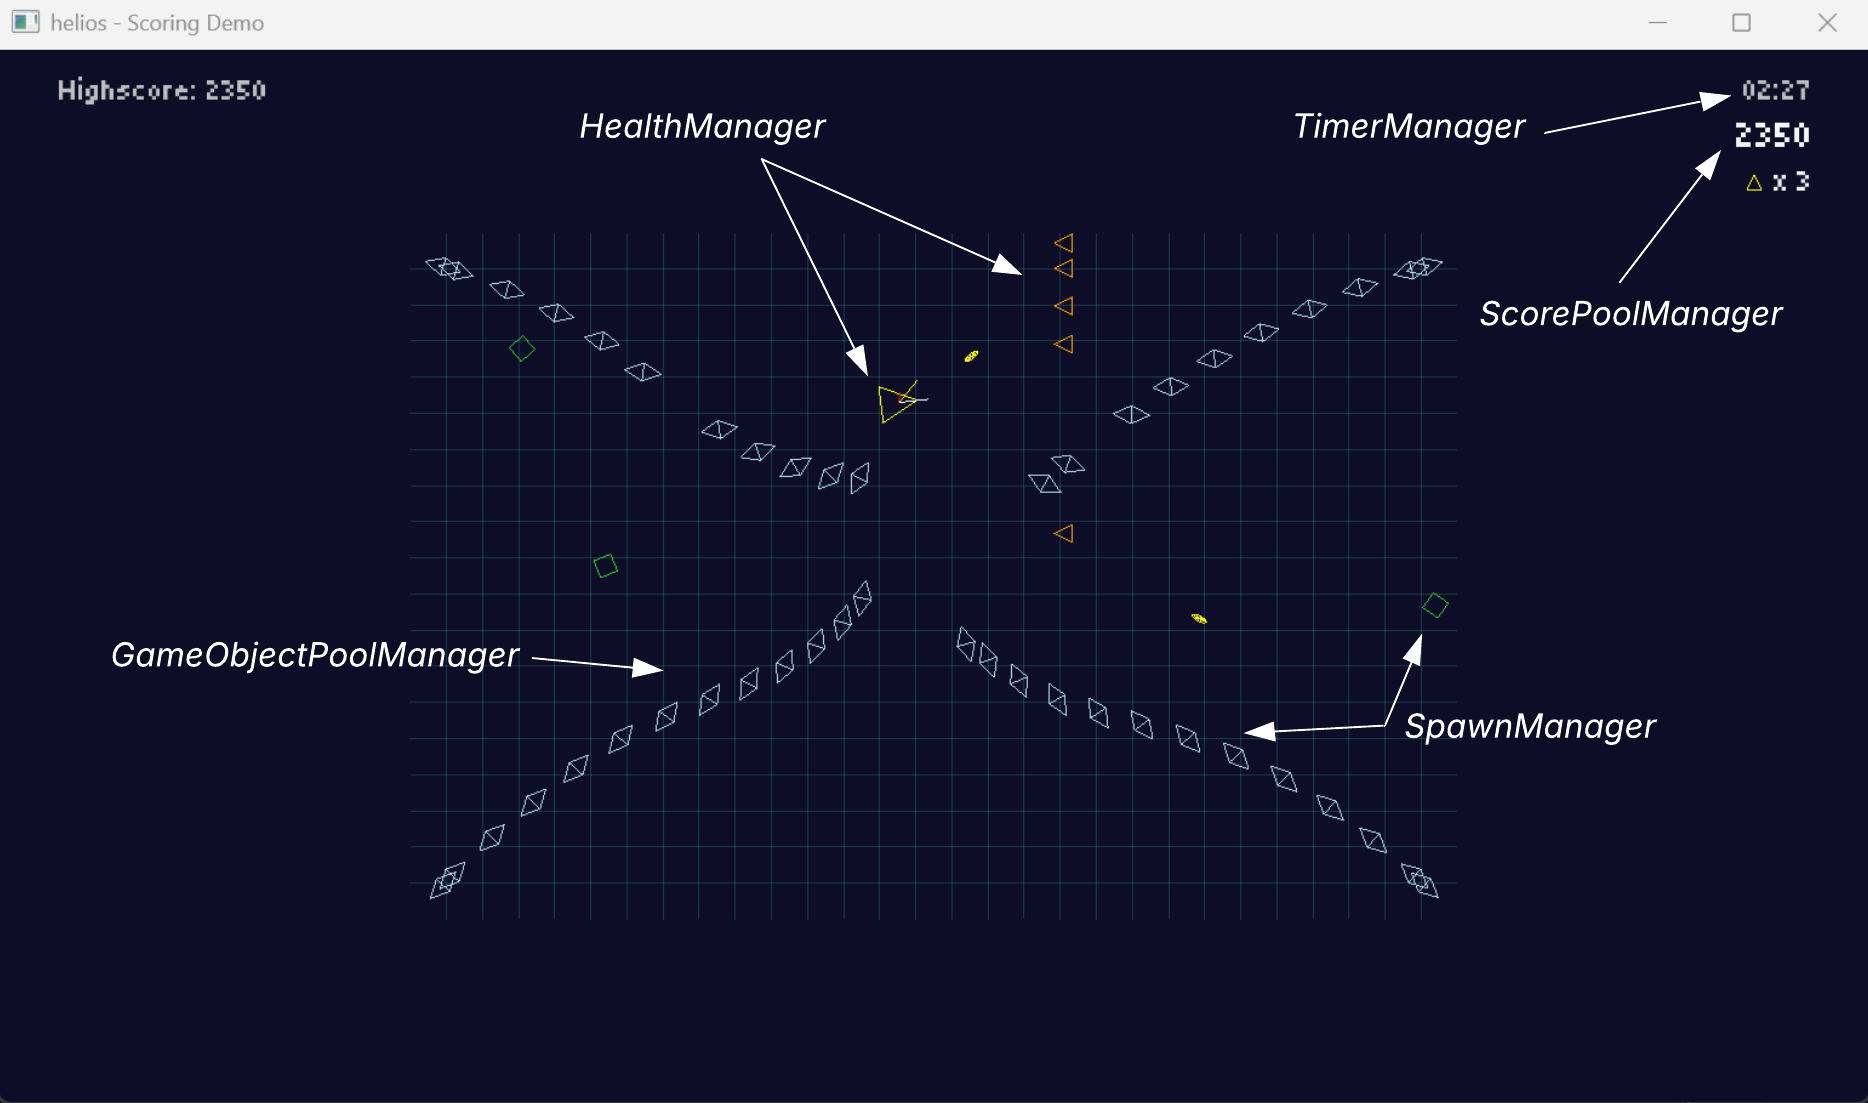
\includegraphics[width=0.8\textwidth]{content/de/architektur/runtime/img/manager.png}
    \caption{Ausschnitt einer Spielszene, in der die Auswirkungen verschiedener Manager auf die Spielwelt dargestellt werden. (Quelle: Eigene Darstellung)}
    \label{fig:manager_auswirkungen}
\end{figure}